\section{Der Morse-Komplex und der Raum der gebrochenen Trajektorien}

Wir sind nun bereit, den Morse-Komplex mit Koeffizienten in $\F_2$ (wenigstens) hinzuschreiben.
Wir fixieren für den \textbf{gesamten Rest der Arbeit}: 
\begin{itemize}
    \item eine glatte \textbf{kompakte} Mannigfaltigkeit $M$.
    \item ein Morse-Smale Paar $(f, X)$.
\end{itemize}
Die Notation, die wir zu Morse-Umgebungen in~\ref{def: notation morse umgebung} entwickelt haben 
wird weiterhin wichtig sein. Definiere $C_k (M, (f, X))$ als das $\F_2$-Modul, 
das von den kritischen Punkten von $f$ mit Index $k$ erzeugt wird, also
\[ C_k = \left\{ \sum_{p \, \in \, \Crit_k (f)} a_p \cdot p : a_p \in \F_2 \right\} . \] 
Außerdem sei 
$n_X(p, q) = \# \Lt (p, q) \mod 2$. Dann definiere für einen kritischen Punkt $p$ mit Index $k + 1$:
\[ \del_X (p) := \sum_{q \, \in \, \Crit_{k}(f)} n_X(p, q)p . \]

Das Ziel dieses Abschnittes ist es zu zeigen, dass der Komplex $C_{\ast}(M, (f, X))$ wohldefiniert
ist, also dass gilt $n_X (p, q) < \infty$, und dass es ein Kettenkomplex ist, also dass 
$\del_X \circ \del_X = 0$. 
% Sobald das gezeigt wurde ist es recht leicht, den Komplex auch über die 
% ganzen Zahlen zu definieren.

\subsection*{Wohldefiniertheit}

\begin{definition}[Der Raum der gebrochenen Trajektorien]
    \label{def: raum der gebrochenen trajektorien}
    Es seien $p$ und $q$ kritische Punkte von $f$. Der \textit{Raum der gebrochenen Trajektorien} ist
    \[ \Lb (p, q) = 
        \bigcup_{k \in \N} \left( \bigcup_{\substack{c_1, \dots, c_{k - 1} \\ \in \Crit(f)}} 
            \Lt (p, c_1) \times \Lt (c_1, c_2) \times \dots 
                \times \Lt (c_{k - 2}, c_{k - 1}) \times \Lt (c_{k - 1}, q) \right) . \]
\end{definition}

Obwohl die Formulierung recht sperrig wirkt ist sie doch intuitiv: 
$\ell \in \Lt (p, q)$ ist eine \glqq Verbindung\grqq{} zwischen den kritischen Punkten $p$ und $q$ 
entlang des Pseudo-Gradientenfeldes $X$. Ein Element 
$(\ell_1, ..., \ell_k) \in \Lt (p, c_1) \times \dots \times \Lt (c_{k - 1}, q) \subseteq \Lb (p, q)$
ist eine \glqq Verbindung\grqq{} zwischen $p$ und $q$ entlang des Pseudo-Gradientenfeldes $X$, die noch 
bei den kritischen Punkten $c_1, \dots, c_{k - 1}$ \glqq Halt\grqq{} macht. 

\begin{figure}[H]
    \centering
    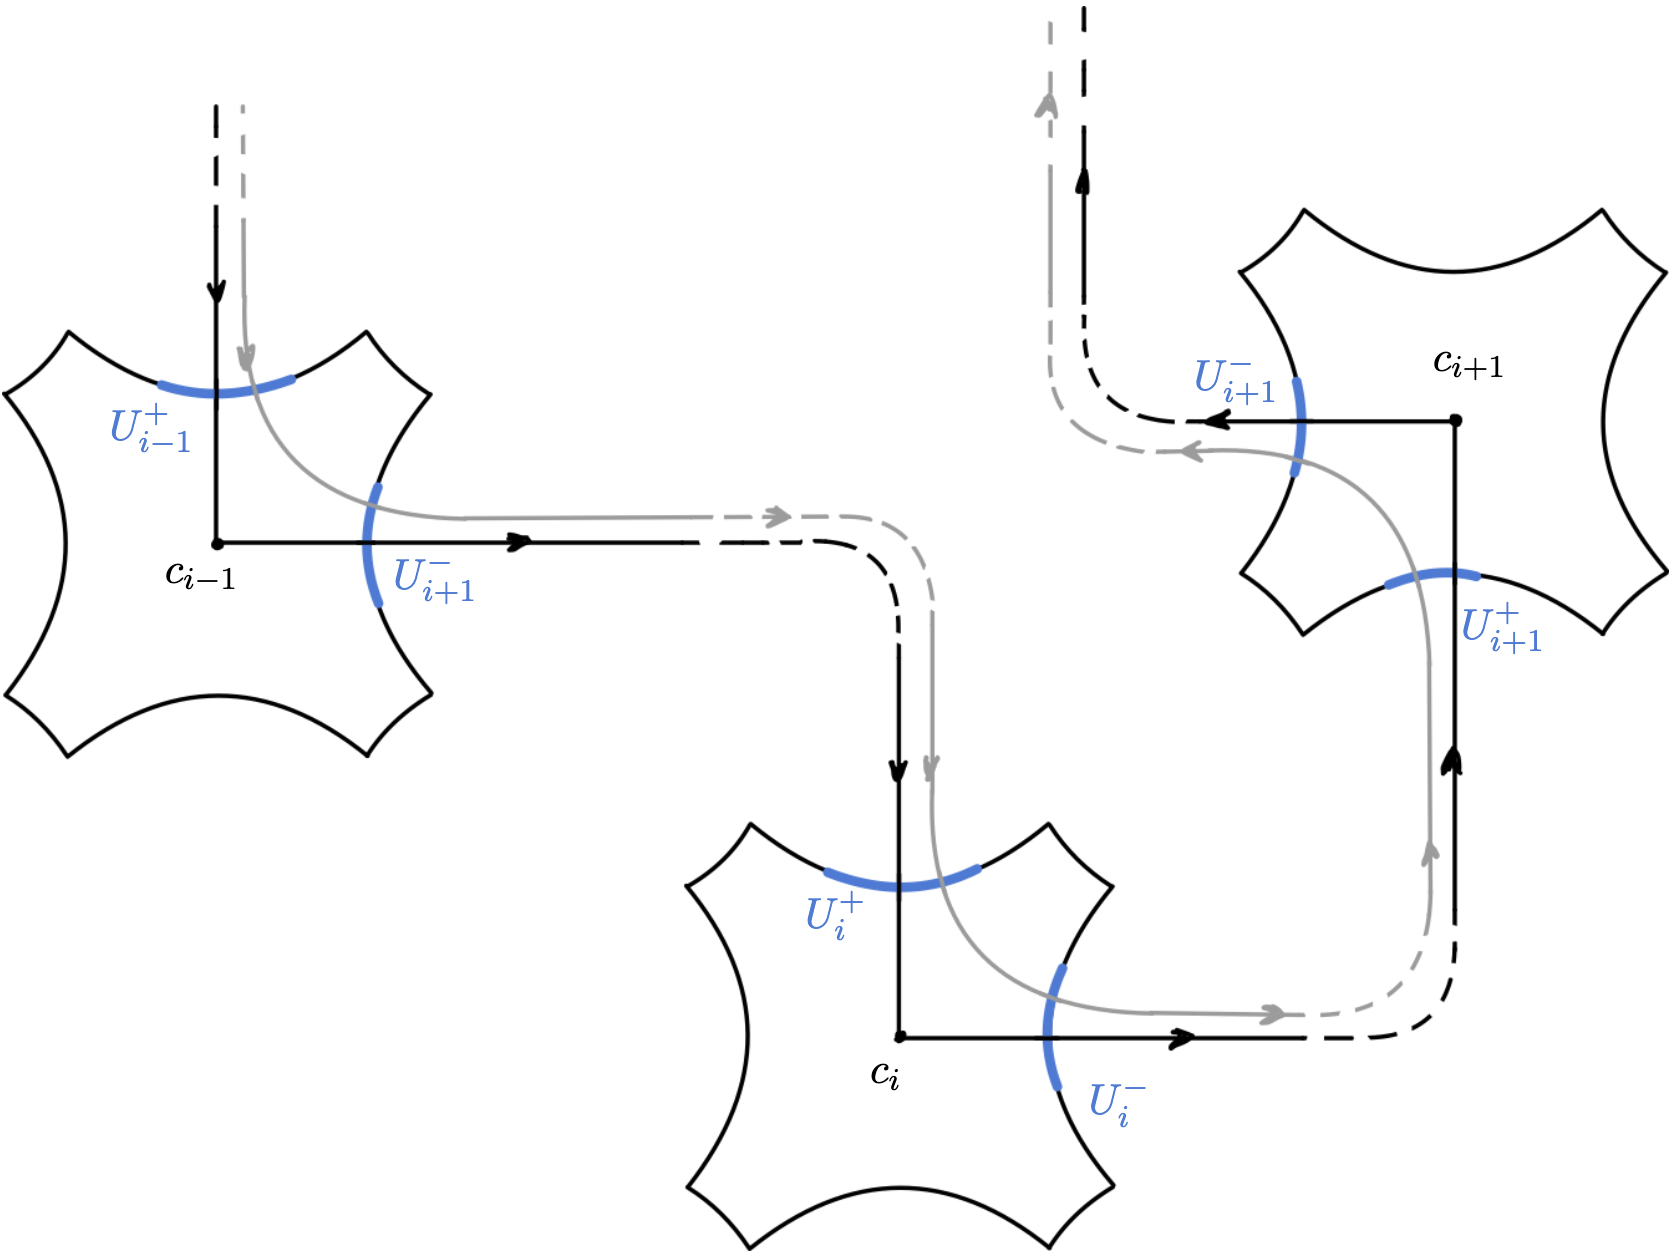
\includegraphics[width=0.5\textwidth]{../resources/broken-trajectories.png}
    \caption{Eine gebrochene Trajektorie (schwarz) und eine nicht gebrochene Trajektorie 
    in einer Umgebung (grau)}
    \label{fig: gebrochene trajektorien}
\end{figure}


Offensichtlich gilt:
\begin{itemize}
    \item Für jedes $\ell \in \Lt (p, c_1) \times \dots \times \Lt (c_{k - 1}, q)$ gilt 
        $\Index (p) < \Index (c_1) < \dots < \Index (c_{k - 1}) < \Index (q)$, denn falls dies nicht
        der Fall ist, ist mindestens einer der Faktoren leer. 
    \item Ist $\Index (p) = \Index (q) + 1$, so ist $\Lb (p, q) = \Lt (p, q)$.
    \item Ist $\Index (p) = \Index (q) + 2$, so ist 
        $\Lb (p, q) = \Lt (p, q) \cup \bigcup_{c \in \Crit (f)} \Lt(p, c) \times \Lt(c, q)$.
\end{itemize}
Tatsächlich sind die beiden letzten Fälle die, die wir am meisten untersuchen werden.
Wir werden sehen, dass man, wie mit der Notation angedeutet, $\Lb (p, q)$ mit einer Topologie 
ausstatten kann, sodass es eine Kompaktifizierung von $\Lt (p, q)$ ist. (In der Tat ist ja 
$\Lt (p, q) \subseteq \Lb (p, q)$).

\begin{definition}[Topologie von $\Lb (p, q)$]
    \label{def: topologie gebrochener trajektorien}
    Wir definieren eine Basis der Topologie von $\Lb (p, q)$. Es seien $p$ und $q$ kritische 
    Punkte von $f$. Wir erinnern uns an unsere Vorstellung von Morse-Umgebungen $\Omega(p)$ wie 
    in~\ref{def: notation morse umgebung}.
    Es sei
    \[ \ell = (\lambda_1, \dots, \lambda_k) 
        \in \Lt (p, c_1) \times \dots \times \Lt(c_{k - 1}, q) \subseteq \Lb (p, q) . \]
    Seien $U_i = \Omega(c_i)$ (nicht unbedingt endgültig gewählte) Morse-Umgebungen von $c_i$ 
    und $U_0$ und $U_k$ Morse-Umgebungen von $p$ und $q$. $\lambda_i \cap \del_+ U_i$ ist der 
    Punkt, an dem $\lambda_i$ in $U_i$ eintritt, und $\lambda_{i + 1} \cap \del_- U_i$ der 
    Punkt, an dem $\lambda_{i + 1}$ die Umgebung $U_i$ verlässt. Es sei $U_i^-$ eine Umgebung von 
    $\lambda_i \cap \del_+ U_i$ in 
    $\del_+ U$ und $U_i^-$ eine Umgebung von $\lambda_{i + 1} \cap \del_- U_i$ in $\del_- U_i$
    (siehe Abb.~\ref{fig: gebrochene trajektorien}). 
    Seien dann $U^- = \bigcup U_i^-$ und $U^+ = \bigcup U_i^+$. Dann definiere ein Element
    $\mathcal{U} (\ell, U^-, U^+)$ aus der Basis wie folgt:

    Wir sagen 
    $\ell' = (\mu_1, ..., \mu_{k'}) \in \Lt (p, c_{i_1}) \times \dots \times \Lt (c_{i_{k'-1}}, q)$
    ist in $\mathcal{U}(\ell, U^-, U^+)$ enthalten, falls $\mu_j \cap U_j^+ \neq \varnothing$
    und $\mu_j \cap U_{j + 1}^- \neq \varnothing$. 

    Eine Menge $\mathcal{V} \subseteq \Lb (p, q)$ heißt dann \textit{offen}, falls $\mathcal{V}$
    die Vereinigung von Elementen aus der Basis ist.
\end{definition}

\begin{remark}
    Die Topologie von $\Lt(p, q)$ als Quotient stimmt mit der von $\Lb(p, q)$ überein.
    Dies ist wieder ersichtlich, wenn wir uns $\Lt (p, q)$ als Schnitt 
    $\mathcal{M} (p, q) \cap f^{-1}(c)$ vorstellen; Die $U^-$ beziehungsweise $U^+$ sind nur 
    offene Umgebungen in den Niveaumengen.
\end{remark}

\begin{prop}
    \label{prop: Lb ist kompakt}
    Es seien $p$ und $q$ kritische Punkte von $f$. Dann ist $\Lb (p, q)$ kompakt.
\end{prop}

Um diese Proposition zu beweisen benötigen wir noch ein Lemma:

\begin{lemma}
    \label{lemma: konvergenz einer folge}
    Es sei $x \in M$ \emph{kein} kritischer Punkt von $f$. Sei außerdem $(x_n)_n$ eine Folge in
    $M$ die gegen $x$ kovnvergiert und seien $y_n$ und $y$ Punkte, die auf den selben Trajektorien
    wie $x_n$ und $x$ liegen. Es gelte außerdem $f(y_n) = f(y)$ für alle $n \in \N$. Dann gilt
    \[ \lim_{n \to + \infty} y_n = y . \]
\end{lemma}

\begin{proof}
    Der Beweis orientiert sich an dem des ersten Deformationslemmas~\ref{satz: erstes deformationslemma}
    (Siehe \cite{audin})
\end{proof}

\begin{proof}[Beweis von Proposition~\ref{prop: Lb ist kompakt}]
    Es sei $(\ell_n)_n$ eine Folge in $\Lb (p, q)$. Um zu zeigen, dass $\Lb (p, q)$ kompakt ist
    müssen wir zeigen, dass $(\ell_n)_n$ eine konvergente Teilfolge besitzt.

    Wir nehmen zuerst an, dass $(\ell_n)_n$ eine Folge in $\Lb (p, q)$ ist.
    Es sei $\ell_n^- \in M$ der Punkt, an dem $\ell_n$ die Morse Umgebung $\Omega(p)$ verlässt 
    und $\ell_n^- \in M$ der Punkt, an dem $\ell_n$ in die Morse Umgebung $\Omega(q)$ eintritt.
    $\ell_n^-$ und $\ell_n^+$ sind im Schnitt von $\del \Omega (p)$ bzw. $\del \Omega (q)$ und 
    der stabilen bzw. instabilen Mannigfaltigkeit. Diese Schnitte sind Kugeloberflächen, also 
    kompakt. Die Folgen $(l_n^-)_n$ und $(\ell_n^+)_n$ haben also konvergente Teilfolgen, wir können 
    demnach ohne Beschränkung der Allgemeinheit annehmen, dass sie konvergent sind. Setze
    \[ \lim_{n \to \infty} \ell_n^- = p^- \text{ und } \lim_{n \to \infty} \ell_n^+ = q^+ . \]
    Sei $\phi$ die von $X$ erzeugte 1-Parameter Gruppe aus Diffeomorphismen, dann ist 
    $\gamma = \phi_{\bullet}(p^-)$ die Trajektorie von $p^-$. Sei 
    $c = \lim_{t \to \infty} \phi_t(p^-)$. Der Punkt $c$ ist nach 
    Proposition~\ref{prop: trajektorien enden in kritischen punkten} ein kritischer Punkt,
    also ist $\gamma \in \Lt (p, c)$.  Es sei $d^+$ der Punkt, an dem $\gamma$ in $\Omega (c)$ 
    eintritt. Da $\phi$ glatt ist, muss wegen der gewählten Topologie 
    aus~\ref{def: topologie gebrochener trajektorien} für $n$ groß genug auch $\ell_n$ die 
    Morse-Umgebung $\Omega (c)$ kreuzen. Sei $d_n^+ \in M$ der Punkt, an dem $\ell_n$ in 
    $\Omega (c)$ eintritt. 
    Dann gilt $d_n^+, d^+ \in \del_+ W$, also gilt $f(d_n^+) = f(d^+)$ für alle $n$. Da $d_n^+$ auf 
    der selben Trajektorie wie $\ell_n^-$ liegt, und $d^+$ auf der selben wie $p^-$,folgt da 
    $\lim \ell_n^- = p^-$ mit dem letzten Lemma~\ref{lemma: konvergenz einer folge}: 
    \[ \lim_{n \to \infty} d_n^+ = d^+ . \]
    Falls $c = q$, dann ist $\lim \ell_n = \gamma \in \Lt (p, q) \subseteq \Lb (p, q)$, also hat 
    dann die Folge $(\ell_n)_n$ eine konvergente Teilfolge. Es sei also $c \neq q$. Dann muss 
    $\ell_n$ die Morse Umgebung $\Omega (c)$ wieder durch einen Punkt $d_n^-$ verlassen. Wie oben 
    können wir ohne Beschränkung der Allgemeinheit annehmen, dass die Folge $(d_n^-)_n$ konvergent 
    ist, da sie zumindest eine konvergente Teilfolge besitzt. Wir definieren dann $d^- := \lim d_n^-$. 
    $d^-$ liegt in der instabielen Mannigfaltigkeit von $c$, denn wäre dies nicht der Fall, dann 
    führt das zu einem Widerspruch:
    
    Angenommen $d^- \notin \unst (c)$. Dann wäre $d^-$ auf der Trajektorie von einem Punkt
    $d^+_{\ast} \in \del_+ \Omega (c)$, der nicht in $\unst (c)$ enthalten ist. Wieder wegen des 
    vorherigen Lemmas~\ref{lemma: konvergenz einer folge} ist dann $\lim d_n^+ = d^+_{\ast}$, also 
    gilt dann $d^+ = d^+_{\ast}$, aber es gilt $d^+ \in \unst (c)$.
    
    Wir können nun wieder mit dem selben Argument zeigen, dass dann die Trajektorie von $d^-$ im
    kritischen Punkt $q$ endet, also liegt dann $\lim \ell_n$ in $\Lt (p, c) \times \Lt (c, q)$.
    \todo{können wir das wirklich?}

    Wir müssen noch zeigen, dass eine Folge $(\ell_n)_n$ in $\Lb (p, q)$ eine konvergente 
    Teilfolge hat. Wegen der Glattheit von $\phi$ können wir annehmen, dass für $n$ groß 
    genug alle $\ell_n$ die Form 
    \[ \ell_n = (\ell^1_n, \dots, \ell^k_n) \in \Lt (p, c_1) \times \dots \times \Lt (c_{k - 1}, q) \]
    haben. Wir finden mit der vorheringen Überlegung komponentenweise eine Teilfolge, sodass wir 
    für den Grenzwert maximal noch $k - 1$ kritische Punkte als \glqq Zwischenstopp\grqq{} einfügen
    müssen. 
\end{proof}

\begin{remark}
    Sind nun $p$ und $q$ kritische Punkte von $f$ mit $\Index (p) = \Index (q) + 1$, dann ist 
    $\Lt(p, q)$ $0$-dimensionale Mannigfaltigkeit. Außerdem ist $\Lt (p, q)$ eine abgeschlossene
    Teilmenge von $\Lb (p, q)$, und wie wir in der letzten Proposition~\ref{prop: Lb ist kompakt}
    gezeigt haben, ist $\Lb(p, q)$ kompakt, also ist auch $\Lt(p, q)$, und somit endlich.
    Damit ist schon mal $n_X (p, q)< \infty$, also $C_k(M (f, X))$ wohldefiniert.
\end{remark}

\subsection*{Der Morse Komplex ist ein Kettenkomplex}

Wir wollen zeigen, dass der Morse-Komplex tatsächlich ein Kettenkomplex ist, also dass 
$\del_X \circ \del_X = 0$.
Wir rechnen:
\begin{align*}
    \del_X (\del_X (p)) = & \del_X (\sum_{c \in \Crit_k (f)} n_X (p, c) \cdot c) \\
    = & \sum_{q \in \Crit_{k - 1}(f)} \left( 
        \sum_{c \in \Crit_k (f)} n_X(p, c) \cdot n_X(c, q) \right) \cdot q
\end{align*}
und 
\[ \sum_{c \in \Crit_k (f)} n_X(p, c) \cdot n_X(c, q) = 
\# \left( \bigcup_{c \in \Crit_k (f)} \Lt (p, c) \times \Lt (c, q) \right) \mod 2 . \]
Es genügt also zu zeigen, dass für kritische Punkte $p$ und $q$ mit Index $k + 1$ und $k - 1$
gilt, dass $\# \left( \bigcup_{c \in \Crit_k (f)} \Lt (p, c) \times \Lt (c, q) \right)$ gerade ist.

Wir benutzen die folgende Aussage, ohne sie zu beweisen:

\begin{theorem}[Klassifizierung kompakter 1-Mannigfaltigkeiten]
    \label{satz: klassifizierung kompakter 1-mannigfaltigkeiten}
    Es sei $M$ eine kompakte zusammenhängende Mannigfaltigkeit mit Rand. Dann ist
    \begin{itemize}
        \item $M$ diffeomorph zu $S^1$, falls $\del M = \varnothing$
        \item $M$ diffeomorph zu $[0, 1]$, falls $\del M \neq \varnothing$
    \end{itemize}
\end{theorem}

\begin{proof}
    Man kann diese Tatsache mithilfe von Morse-Theorie beweisen, wie es Audain und Damian in 
    \cite{audin} tun, aber ein einfacherer Beweis ist bei Milnor in \cite{milnor2} zu finden.
\end{proof}

\begin{theorem}
    \label{satz: gebrochene trajektorien sind 1-dim mannigfaltigkeit}
    Es seien $p$ und $q$ kritische Punkte von $f$ mit $\Index (p) = k + 1$ und $\Index (q) = k - 1$
    für ein $k \in \N_0$. Dann ist $\Lb (p, q)$ eine 1-dimensionale Mannigfaltigkeit mit Rand, und das
    Innere von $\Lb (p, q)$ ist $\Lt (p, q)$.
\end{theorem}

Mit dieser Proposition folgt dann mit der Klassifizierung von $1$-Mannigfaltigkeiten mit 
Rand~\ref{satz: klassifizierung kompakter 1-mannigfaltigkeiten} schon, dass der Morse Komplex ein
Kettenkomplex ist, denn dann ist 
\[ \# \left( \bigcup_{c \in \Crit (f)} \Lt (p, c) \times \Lt (c, q) \right) = \del \Lb (p, q) \]
gerade.

\begin{bigproof}
    Wir wissen schon, dass $\Lt (p, q) \subseteq \Lb(p, q)$ eine $1$-dimensionale Mannigfaltigkeit ist. 
    Um sagen zu können, dass $\Lb (p, q)$ eine $1$-dimensionale Mannigfaltigkeit mit Rand ist, und 
    insbsondere, dass $\Lt (p, q)$ das Innere von $\Lb(p, q)$ ist, reicht die folgende Aussage über 
    $\Lb(p, q)$:
    Es sei $c$ ein weiterer kritischer Punkt mit Index $k$.
    Sei $\lambda_1 \in \Lt (p, c)$ und $\lambda_2 \in \Lt (c, q)$. Dann existiert eine offene Umgebung
    $U \subseteq \Lb (p, q)$ von $(\lambda_1, \lambda_2)$, ein $\delta > 0$ und eine (topologische)
    Einbettung $\psi \colon [0, \delta) \to U$, sodass gelten: 
    \begin{enumerate}
        \item $\psi|_{(0, \delta)}$ ist glatt eine glatte Einbettung.
        \item $\psi(0) = (\lambda_1, \lambda_2)$.
        \item $\psi((0, \delta)) \subseteq \Lt (p, q)$.
        \item Für jede Folge $(\ell_n)_n$ in $\Lt (p, q)$ die gegen $(\lambda_1, \lambda_2)$ konvergiert 
            gilt $\ell_n \in \Ima \psi$ für $n$ groß genug.
    \end{enumerate} 
    Die letzte Bedingung stellt sicher, dass sich in $(\lambda_1, \lambda_2)$ keine 
    \say{Kreuzung} befindet (wie zum Beispiel der Klebepunkt bei $S^1 \vee S^1$).
    Wir begeben uns also auf die (recht lange) Suche nach einer solchen Abbildung $\psi$. 

    Wir machen ein Paar Konstruktionen. Sei $\alpha := f(c)$ und $(V, \kappa)$ eine Morse Karte von
    $c$, $\Omega(c)$ wie in der Notation zu Morse Umgebungen~\ref{def: notation morse umgebung}. 
    Dann sind $f(\del_+ \Omega (c)) = \alpha + \eps$ und $f(\del_- \Omega (c)) = \alpha - \eps$ für ein 
    $\eps > 0$. Außerdem setze
    \begin{align*}
        S_+ (c) := & \stab (c) \cap f^{-1}(\alpha + \eps) \diffeo S^{n - k - 1} \\
        S_- (c) := & \unst (c) \cap f^{-1}(\alpha - \eps) \diffeo S^{k - 1} .
    \end{align*}
    Dass $S_+ (c)$ und $S_- (c)$ diffeomorph zu Sphären sind hatten wir schon vorher gesehen.
    Es sei $a_1 \in M$ der Punkt, an dem $\lambda_1$ auf $\Omega(c)$ trifft, also 
    $a_1 = S_+ (c) \cap \lambda_1$, und $a_2$ der Punkt, an dem $\lambda_2$ die Umgebung $\Omega (c)$ 
    wieder verlässt, also $a_2 = S_- (c) \cap \lambda_2$. $\alpha + \eps$ ist kein kritischer Wert 
    von $f$ und es gilt $f^{-1}(\alpha + \eps) \pitchfork \unst (p)$, also ist mit 
    Proposition~\ref{prop: schnitt von transversalen untermannigfaltigkeiten} 
    $P = f^{-1}(\alpha + \eps) \cap \unst (p)$ eine Mannigfaltigkeit mit Dimension 
    $(n - 1) + (k + 1) - n = k$. Da $X$ die Smale-Eigenschaft erfüllt, $P \subseteq \unst (p)$,
    $S_+ \subseteq \stab(c)$, $P, S_+(c) \subseteq f^{-1}(c + \eps)$ und 
    $\dim P + \dim S_+(c) = n - 1$, gilt $P \pitchfork S_+ (c)$. Also ist $P \cap S_+ (c)$
    mit Proposition~\ref{prop: schnitt von transversalen untermannigfaltigkeiten} eine 
    Untermannigfaltigkeit der Dimenion $k + (n - k - 1) - (n - 1) = 0$. Offensichtlich gilt 
    $a_1 \in P \cap S_+ (c)$. Es sei $B^k_{\delta} = \{ x \in \R^k : \| x \| < \delta \}$. Dann 
    existiert eine Umgebung $B$ von $a_1$ in $P$ und ein Diffeomorphismus 
    $\Psi : B \longto B^k_{\delta}$ mit $\Psi(a_1) = 0$, sodass $B \cap S_+ (c) = a_1$ 
    und $B \subseteq \del_+ \Omega (c)$. Wir versuchen die Kernidee des Beweises zu verstehen:

    \begin{figure}
        \centering
        \begin{tikzpicture}
            % Include the image in a node
            \node [
                above right,
                inner sep=0] (image) at (0,0) {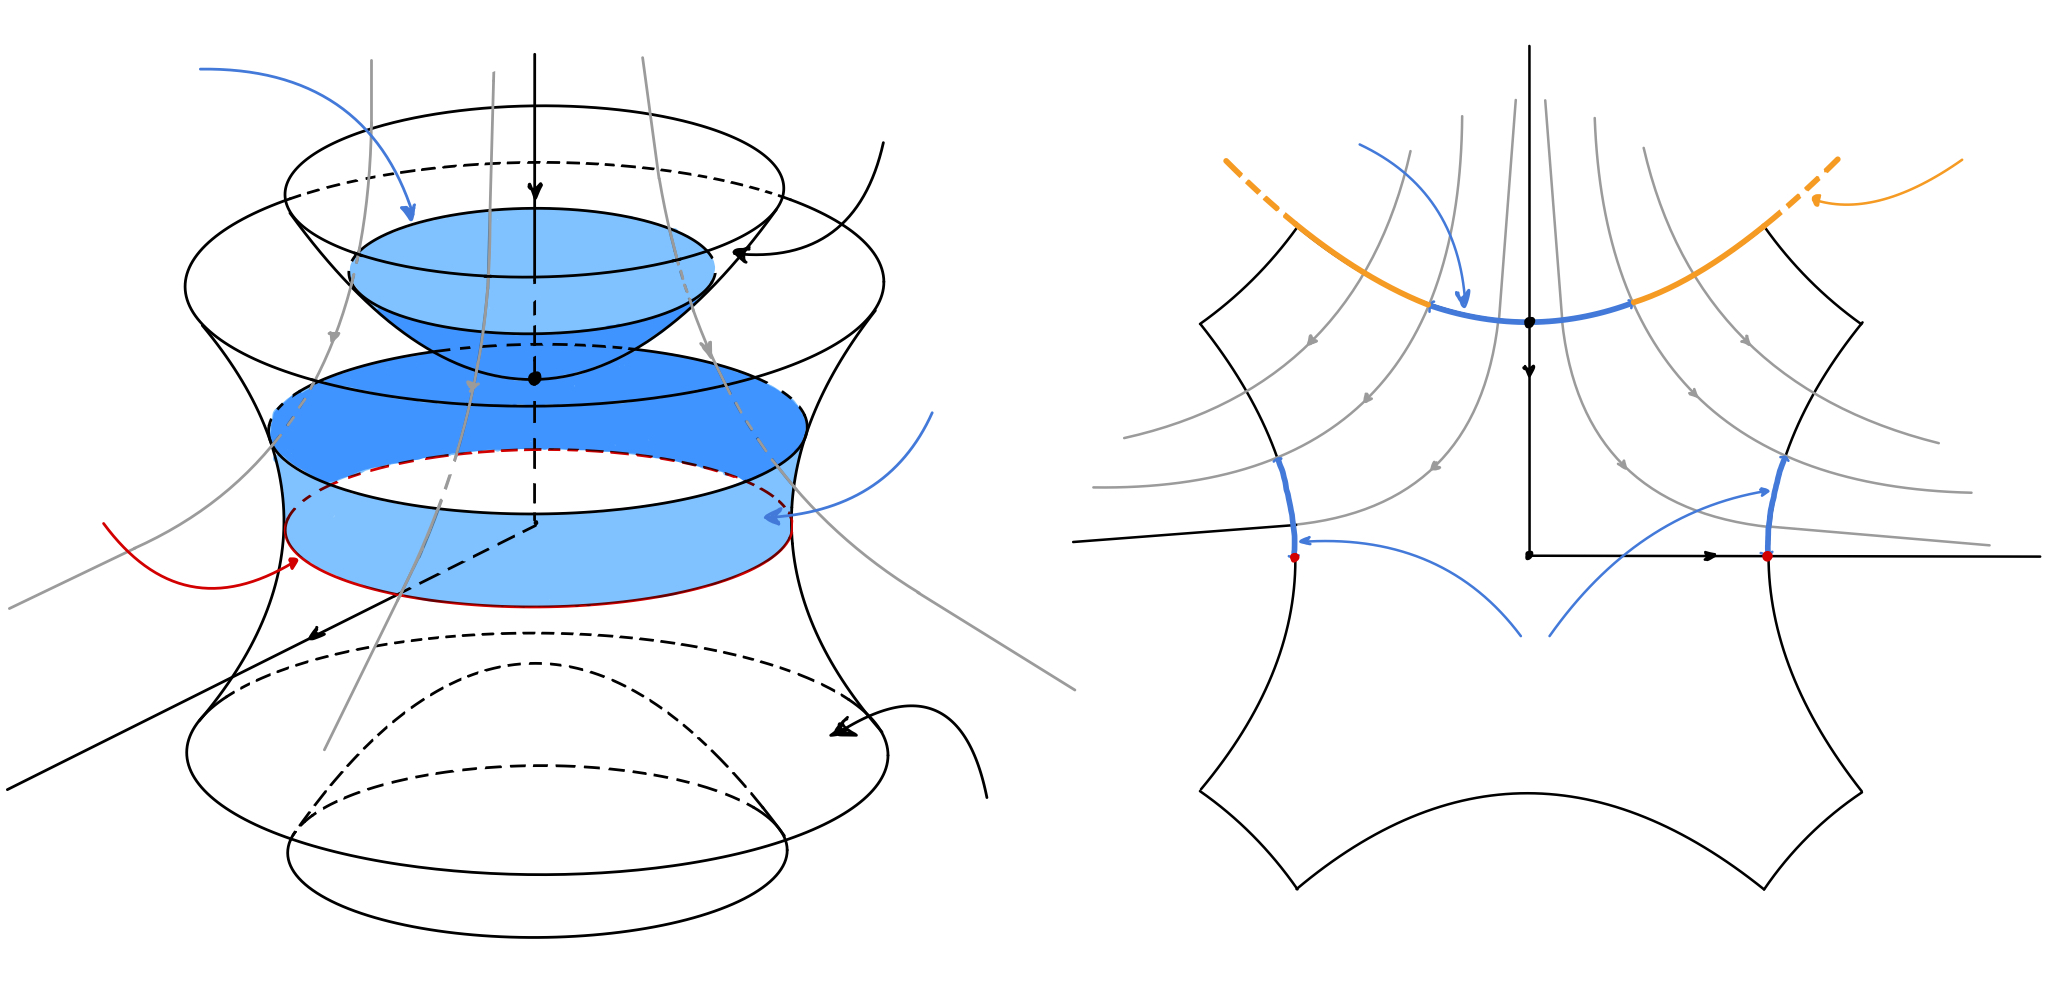
\includegraphics[width=\textwidth]{../resources/lb-ist-1-dim-mfkt.jpeg}};
                
            % Create scope with normalized axes
            \begin{scope}[
            x={($0.02*(image.south east)$)},
            y={($0.05*(image.north west)$)}]
            
            % Annotate left figure
            \node at (13.2, 9.1) {\tiny $c$};
            \node at (13.2, 12.1) {\tiny $a$};

            \node at (13.5, 18.7) {\tiny $\lambda_1$};
            \node at (3.2, 4.8) {\tiny $\lambda_2$};
            
            \node[text=red] at (2.5, 10.1) {\tiny $S_- (c)$};

            \node[text=LightBlue] at (4, 18.5) {\tiny $B$};
            \node[text=LightBlue] at (22.5, 12.3) {\tiny $\Ima (\Phi)$};
        
            \node at (21.5, 17.8) {\tiny $f^{-1}(\alpha + \eps)$};
            \node at (23.8, 3.6) {\tiny $f^{-1}(\alpha - \eps)$};
            
            % Annotate right figure
            \node at (36.6, 8.6) {\tiny $c$};
            \node at (36.5, 13.2) {\tiny $a$};

            \node at (37.6, 18.5) {\tiny $\lambda_1$};
            \node at (48.5, 8.4) {\tiny $\lambda_2$};

            \node[text=red] at (32.4, 8.2) {\tiny $S_-(c)$};
            
            \node[text=LightBlue] at (32.4, 17.4) {\tiny $D$};
            \node[text=LightBlue] at (37, 6.8) {\tiny $\Ima (\Phi)$};

            \node[text=orange] at (47.8, 17.2) {\tiny $P$};
            
            % \draw[lightgray,step=1] (image.south west) grid (image.north east);
            \end{scope}
        \end{tikzpicture}
        \caption{Anschauung von $\Phi$, falls $\Index (c) = 1$ und $M$ $3$-dimensional 
        (links) und $2$-dimensional (rechts)}
        \label{fig: anschauung von phi}
    \end{figure}

    Man betrachte die Abbildungen~\ref{fig: anschauung von phi}.

    Wir versuchen, die Menge $B - a_1$ entlang der Trajektorien von $X$ auf $\del_- \Omega(c)$ via einer 
    Abbildung $\Phi$ einzubetten. Wir werden sehen, dass $Q = \Ima (\Phi) \cup S_+(c)$ eine 
    Mannigfaltigkeit mit Rand ist, und dass dann $Q \cap \stab (q)$ eine $1$-dimensionale
    Mannigfaltigkeit mit Rand ist, und $a_2 \in \del (Q \cap \unst (q))$. Wie 
    in~\ref{prop: wohldefiniertheit von Lt} ist $Q \cap \stab (q) - a_2$ eine Teilmenge von 
    $\Lt (p, q)$, und $a_2 \in \Lt (c, q)$, wenn wir also $a_2 \in \lambda_2$ mit 
    $(\lambda_1, \lambda_2)$ identifizieren, dann bekommen wir unsere Parametrisierung 
    $\psi$ von $\Lb (p, q)$. 
    Also:

    \begin{claim}
        Es sei $\phi$ die von $X$ erzeugte 1-Parameter Gruppe aus Diffeomorphismen. Für jedes 
        $x \in B - a_1$ existiert ein $t_x \in \R$, sodass $\phi_{t_x} (x) \in \del_- \Omega (c)$
        und $x \mapsto t_x$ glatt ist.
    \end{claim}

    \begin{smallproof}
        Via unserer anfangs gewählten Morse Karte $(V, \kappa)$, und da wir ohne Einschränkungen $B$ 
        klein genug wählen können, sodass $B \subseteq \Omega (c)$, können wir annehmen, dass sich 
        alles im $\R^n$ abspielt ; Sei also ohne Beschränkung der Allgemeinheit 
        $f(x_-, x_+) = - \|x_-\| + \|x_+\|$. Dann ist $\phi$ gegeben durch 
        \[ \phi_t(x_-, x_+) = (e^{2t}x_-, e^{-2t}x_+) . \]
        Falls $(x_-, x_+) \in \del_+ U$ und $x_- \neq 0$, dann gilt auch $x_+ \neq 0$. Setze
        \[ t_{(x_-, x_+)} = \frac{1}{2} \ln \left( \frac{\| x_+ \|}{\| x_- \|} \right) . \]
        Dann gilt
        \[ \phi_{t_{(x_-, x_+)}} (x_-, x_+) = 
            \left( \frac{\| x_+ \|}{\| x_- \|} x_-, \frac{\| x_- \|}{\| x_+ \|} x_+ \right) . \]
        Die Zuordnung $(x_-, x_+) \mapsto t_{(x_-, x_+)}$ ist glatt und 
        \begin{align*}
            f(\phi_{t_{(x_-, x_+)}})(x_-, x_+) = & - \| \frac{\| x_+ \|}{\| x_- \|} x_- \|
                +  \| \frac{\| x_- \|}{\| x_+ \|} x_+ \| \\
                = & - \| x_+ \| + \| x_- \| \\
                = & - \eps .
        \end{align*}
        Es folgt $\phi_{t_{(x_-, x_+)}} (x) \in \del_- U$.
    \end{smallproof}

    Wir haben nun also eine Einbettung $\Phi$ von $B - a_1$ entlang der Trajektorien von $X$ gefunden.
    Wie am Anfang besprochen wollen wir jetzt zeigen:

    \begin{claim}
        Ist $\delta$ klein genug, dann ist $Q = \Ima (\Phi) \cup S_+ (c)$ eine $k$ dimensionale 
        Mannigfaltigkeit mit Rand, und es gilt $\del Q = S_- (c)$.
    \end{claim}

    \begin{smallproof}
        Wieder spielt sich alles via $\kappa$ im $\R^n$ ab. Sei wie 
        in~\ref{def: notation morse umgebung} $U = \kappa^{-1}(\Omega (c))$.
        Man betrachte die Projektion
        \[ \pi \colon \R^k \times \R^{n - k} ; \pi (x_-, x_+) = x_- . \]
        und ihre Einschränkung $\del_+ U \to B_{\eta}^k$.
        \todo{weiß net ob das stimmt, naja} Da $S_+ := \kappa(S_+(c)) = (\pi|_{\del_+U})^{-1}(0)$
        und $B \pitchfork S_+$, ist $0$ ein regulärer Wert von $\pi|_{\del_+U}$.
        Also ist $\opd ( \pi|_{\del_+U} )(0)$ surjektiv, und da dim $\del_+U = k = \dim B^k_{\delta}$ ist
        das Differential auch invertierbar. Jetzt können wir den Satz über die Umkehrfunktion anwenden 
        und bekommen lokal ein Inverses der Abbildung $\pi|_{\del_+U}$. Es existiert also ein 
        $\delta' \leq \eta$, sodass das Inverse von $\pi|_{\del_+U}$ auf $B^k_{\delta'}$ definiert 
        ist. Dann ist 
        \begin{align*}
            (\pi|_{\del_+U})^{-1} \colon B^k_{\delta'} \longto & B \\
            x_- \longmapsto & (x_-, x_+) =: (x_-, h(x_-))
        \end{align*}
        ein Diffeomorphismus. Da $B \subseteq \del_+U \subseteq f^{-1}(\eps)$, gilt dann 
        $\| h(x_-) \|^2 = \| x_- \|^2 + \eps $. Ist dann 
        $g = \cfrac{h}{\| h \|} \colon B^k_{\delta'} \to S^{n - k - 1}$, dann gilt
        \[ B = \{ (x_-, h(x_-)): x \in B^k_{\delta'} \} 
            = \{ (x_-, \sqrt{\| x_- \|^2 + \eps} \cdot g(x_-)): x \in B^k_{\delta'} \} . \]
        Dann bekommen wir mit der Einbettung aus Behauptung 1 und da $\| g(x_-) \| = 1$:
        \[ \Phi(B - a_1) = 
            \left\{ \left( \frac{\sqrt{\| x_- \|^2 + \eps}}{\| x_- \|} \, x_-, \; 
                    \| x_- \| \, g(x_-) \right) : 
                x_- \in B^k_{\delta'} - 0 \right\} \]
        Wir können nun auf $B^k_{\delta'} - 0$ Polarkoordinaten anwenden. wir erhalten eine 
        Einbettung
        \begin{align*}
            H = \Phi^{-1} \circ \rho \colon (0, \delta') \times S^{k-1} \longto & \del_- U \\
            (r, v) \longmapsto & ( \sqrt{r^2 + \eps} \cdot v, r \cdot g(\rho(r, v))) .
        \end{align*}
        $g$ ist auf ganz $B^k_{\delta'}$ definiert, und wenigstens in einer Umgebung von $0$ 
        beschränkt. Also können wir $H$ stetig in $0$ durch
        \[ H(0, v) = (\sqrt{\eps} \cdot v, \, 0) \]
        fortsetzen. Dann ist $H$ auch weiterhin eine (topologische) Einbettung mit 
        $\Ima (H) = \Ima (\Phi) \cup S_- $, und es gilt 
        \[ H(0, S^{k - 1}) = S_- . \]
    \end{smallproof}

    Wir wissen, dass für $f(q) < \alpha - \eps < f(c)$ gilt 
    $\Lt (c, q) \diffeo \mathcal{M} (p, q) \cap f^{-1}(\alpha - \eps)$. 
    
    Außerdem gilt $\stab (q) \pitchfork \Ima \Phi$ und $\stab (q) \pitchfork S_-(c)$ in 
    $f^{-1}(\alpha - \eps)$, also ist mit 
    Proposition~\ref{prop: schnitt von transversalen untermannigfaltigkeiten}
    $\stab (q) \cap Q$ eine Mannigfaltigkeit mit Rand der Dimension $(n - (k - 1)) + k - n = 1$,
    und der Rand von $\stab (q) \cap Q$ ist $\stab (q) \cap S_-(c) \subseteq \Lt (c, q)$, also ist 
    $a_2 \in \del (\stab(q) \cap Q)$.

    Wähle eine Parametrisierung von einer Umgebung von $a_2$ in $\stab (q) \cap Q$
    \[ \chi \colon [0, \delta) \to \stab (q) \cap Q . \]
    Es gilt dann $\chi(0) = a_2$.
    
    Damit erhalten wir die Abbildung 
    \[ \Phi^{-1} \circ \chi \colon (0, \delta) \longto \stab (q) \cap (D - a_1) \subseteq \Lt (p, q) . \]
    Definiere nun 
    \begin{align*} 
        \psi \colon [0, \delta) \longto & \Lb (p, q) \\
        t \longmapsto & \begin{cases}
            \Phi^{-1} \circ \chi (t) & \text{ falls } t \neq 0 \\
            (\lambda_1, \lambda_2) & \text{ falls } t = 0
        \end{cases}
    \end{align*}
    Wir wollen zeigen, dass $\psi$ die gewünschten Eigenschaften vom Anfang erfüllt.

    Offensichtlich ist $\psi$ bijektiv. $\psi$ ist stetig, denn ist $(x_n)_n$ eine Folge in 
    $(0, \delta)$, die gegen $0$ konvergiert, dann konvergiert die Folge $(\chi(x_n))_n$ in 
    $\stab (q) \cap Q \subseteq \del_- \Omega (c)$ gegen $a_2$. Dann folgt aus dem 
    Lemma~\ref{lemma: konvergenz einer folge}, dass die  Folge $(y_n)_n$ in $\stab (q) \cap (B - a_1)$
    mit $y_n = \Phi^{-1}(\chi(x_n))$ gegen $a_1$ konvergiert, also konvergiert $\psi(x_n)$ gegen
    $(\lambda_1, \lambda_2)$. Genau dasselbe gilt für die Umkehrabbildung:

    Ist $(x_n)_n$ eine Folge in $\stab (q) \cap B$, die gegen $a_1$ konvergiert, dann konvergiert
    $\Phi (x_n)$ gegen $a_2$, also $\chi^{-1} (\Phi(x_n))$ gegen $0$.
    Also ist die Abbildung $\psi$ ein Homeomorphismus, und die drei Bedingungen, die an $\psi$ gestellt
    werden, sind offensichtlich aufgrund der Konstruktion erfüllt. 

    Wir müssen nur noch 4. zeigen.

    Sei $(\ell_n)_n$ eine Folge in $\Lt (p, q)$, die gegen $(\lambda_1, \lambda_2)$ konvergiert. 
    Für $n$ groß genug können wir annehmen, dass die $\ell_n$ die Morse Umgebung $\Omega (c)$ betreten 
    und verlassen. Seien wieder wie vorher die $\ell_n^+ = \ell_n \cap \del_+ \Omega (c)$ die Punkte, 
    an denen $\ell_n$ die Umgebung $\Omega (c)$ verlässt und $\ell_n^- = \ell_n \cap \del_- \Omega (c)$
    die Punkte, an denen $\ell_n$ in die Umgebung $\Omega (c)$ eintritt. Wegen der Topologie, die wir 
    auf $\Lb(p, q)$ definiert haben gilt offensichtlich
    \[ \lim_{n \to \infty} \ell_n^- = a_1 \; \; \text{ und } \; \; \lim_{n \to \infty} \ell_n^+ = a_2 , \]
    und da $\Phi$ den Trajektorien von $X$ folgt gilt $\Phi(\ell_n^-) = \ell_n^+$.
    Für $n$ groß genug gilt also $\ell_n^- \in D - a_1$, also $\ell_n^+ \in Q$. Sowieso gilt schon, dass
    $\ell_n^+ \in \stab (q)$, also 
    \[ \ell_n^- \in Q \cap \stab (q) = \Ima \chi . \]
    Hier betrachten wir wieder $\Lt (p, q)$ als $\mathcal{M} (p, q) \cap f^{-1} (\alpha + \eps)$.
    Außerdem ist $\Phi^{-1}(\ell_n^+) = \ell_n^-$, also $\ell_n \in \Ima (\psi)$.
\end{bigproof}

\begin{definition}[Morse-Homologie]
    \label{def: morse-homologie}
    Die \textit{Morse-Homologie} ist die Homologie des Morse-Komplexes. Ist also
    \[ \del_X^k := \del_X \colon C_k (M, (f, X)) \longto C_{k - 1} (M, (f, X)), \]
    dann ist die Morse Homologie im $k$-ten Grad 
    \[ HM_k (M, (f, X)) = \frac{\Ker \, \del_X^k}{\Ima \, \del_X^{k + 1}} \]
\end{definition}

Wir haben gezeigt, dass $(C_{\ast}(M, (f, X)), \del_X)$ ein Kettenkomplex ist, also ist die 
Morse-Homologie wohldefiniert.

\begin{example}
    Wir können uns wieder unser Bespiel einer Morse-Funktion auf dem Torus, die die Smale-Bedingung 
    erfüllt anschauen, also die mit Vorschrift $f(x, y) = -\cos (\pi \cdot x) - \cos(\pi \cdot y)$.
    Zwar ist der Gradient kein Pseudo-Gradientenfeld, denn er erfüllt nicht die zweite Bedingung,
    aber wir könnten $f$ leicht verändern, sodass der Gradient ein Pseudo-Gradient ist, und sodass
    sich die anderen Untersuchten Eigenschaften nicht wesentlich verändern.
    Hier noch einmal die Höhenlinien und der Fluss des Gradientens:
    \begin{figure}[H]
        \centering
        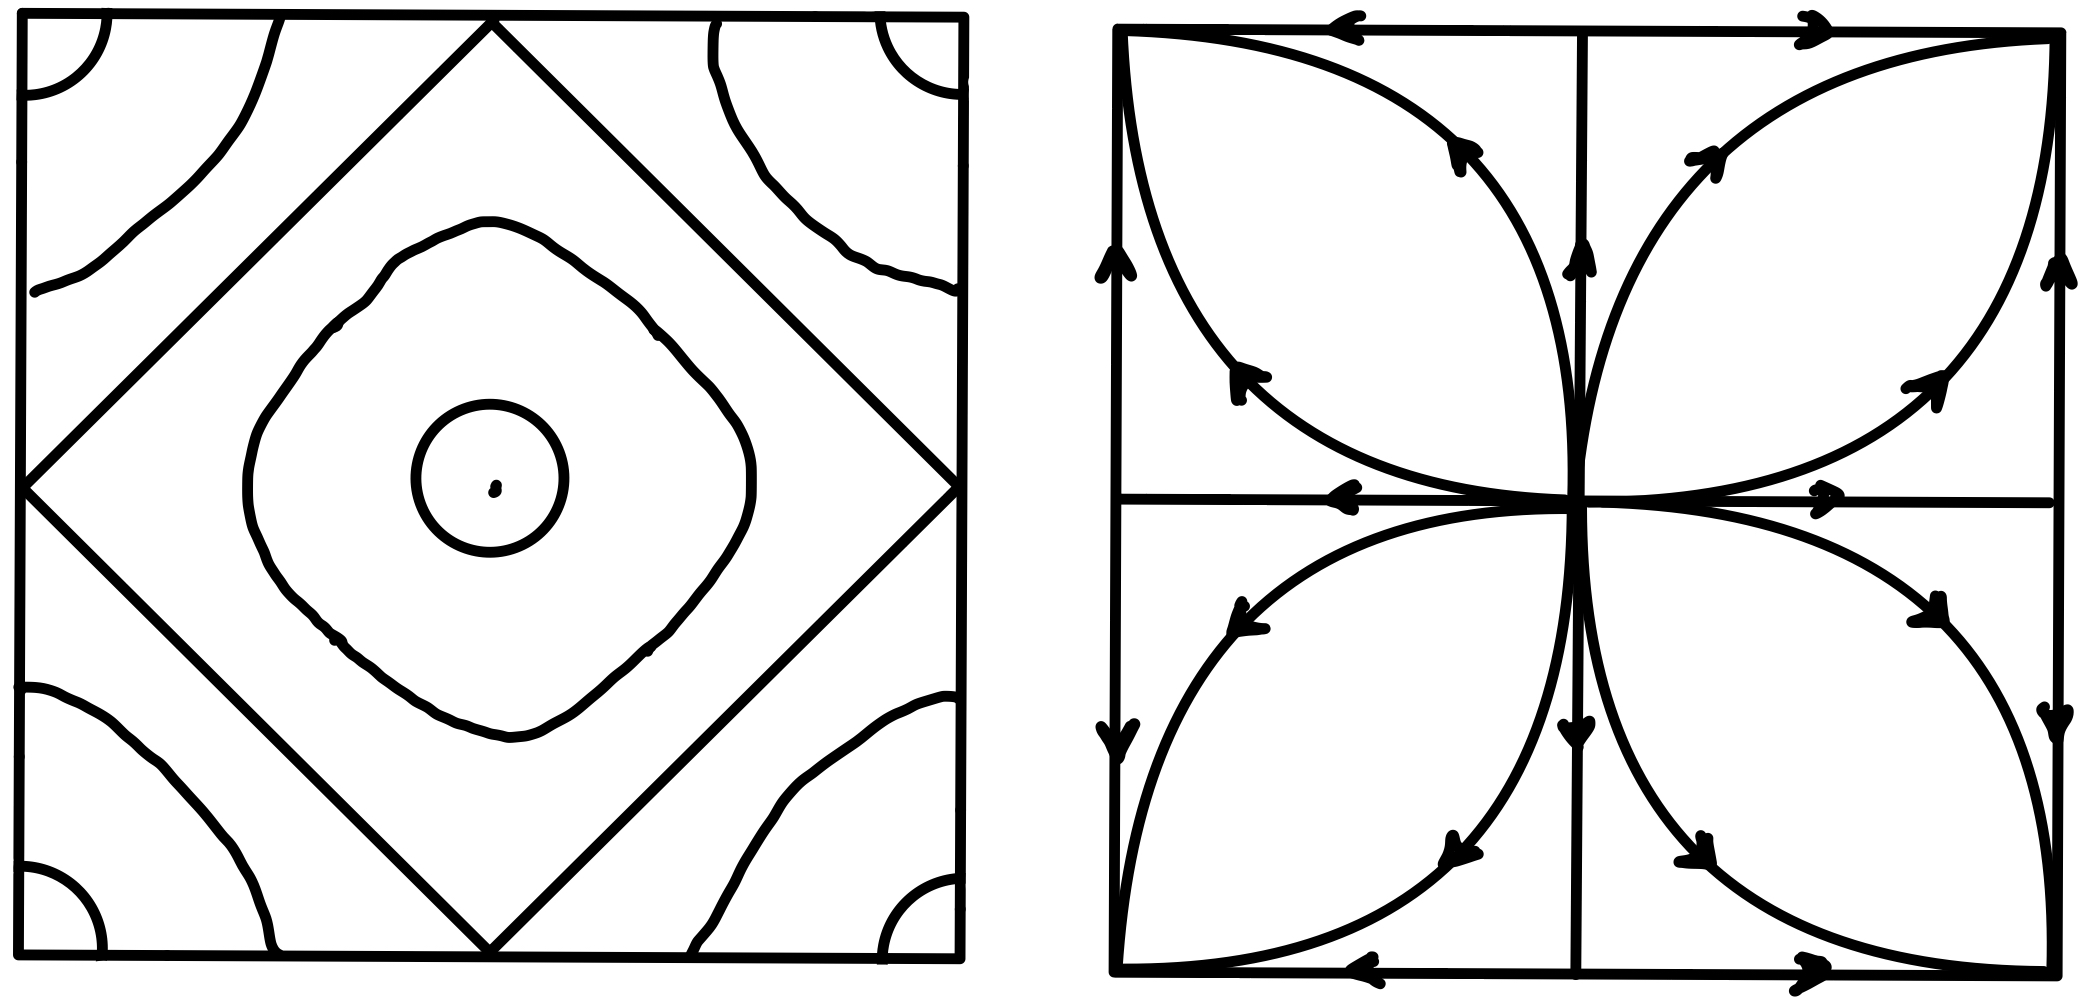
\includegraphics[width=0.4\textwidth]{../resources/morse-funktion-torus.jpeg}
    \end{figure}
    Der Punkt $p = (\sfrac{1}{2}, \sfrac{1}{2})$ ist ein Maximum, die beiden Punkte 
        $c_1 = (0, \sfrac{1}{2}) = (1, \sfrac{1}{2})$ und $c_2 = (\sfrac{1}{2}, 0) = (\sfrac{1}{2}, 1)$
        sind Sattelpunkte und der Eckpunkt $q$ ist ein Minimum. Von $p$ gehen zwei Trajektorien jeweils
        zu $c_1$ und $c_2$ und von $c_1$ und $c_2$ gehen jeweils zwei Trajektorien zu $q$. Der Morse-
        Komplex ist also der folgende:
        \[ \begin{tikzcd}[row sep=tiny]
            \text{Grad:} & 3 & 2 & 1 & 0 & -1 \\
            & 0 \arrow[r, "0"] & \F_2 \arrow[r, "0"] & \F_2^2 \arrow[r, "0"] & \F^2 \arrow[r, "0"] & 0
        \end{tikzcd} \]
        Dann ist 
        \[ HM_k = \begin{cases}
            0 & \text{ falls } k > 2 \text{ oder } k < 0 \\
            \F_2 & \text{ falls } k = 0 \text{ oder } k = 2 \\
            \F_2^2 & \text{ falls } k = 1
        \end{cases} \]
\end{example}

% \subsection*{Der Morse Komplex über \texorpdfstring{$\Z$}{TEXT}}

% Wir haben nun den Morse Komplex über $\F_2$ definiert. Wir wollen noch allgemeiner einen Komplex
% über $\Z$ definieren. Die meiste Arbeit dafür ist nun schon gemacht. Um den Morse-Komplex über 
% $\Z$ zu definieren, wollen wir den Raum der Trajektorien $\Lt (p, q)$ orientieren. Dafür beschäftigen 
% wir uns ein wenig mit Orientierungen von Vektorräumen.

% \begin{definition}[Orientierung und Koorientierung]
%     Es sei $V$ ein endlich dimensionaler Vektorraum. Seien außerdem $\B_1$ und $\B_2$ Basen von $V$. 
%     Definiere
%     \[ \B_1 \sim_O \B_2 \Longleftrightarrow \det \, _{\B_1}[\id_V]_{B_2} > 0 \]
%     Man rechnet leicht nach dass $\sim_O$ eine Äquivalenzrelation ist und dass es bezüglich $\sim_O$
%     genau zwei Äquivalenzklassen gibt.
%     Zwei Basen heißen \textit{gleich orientiert} wenn sie äquivalent bezüglich $\sim_O$ sind. 
%     Eine \textit{Orientierung} ist eine Wahl der Äquivalenzklasse. Ein \textit{orientierter Vektorraum} 
%     ist ein Vektorraum zusammen mit einer Orientierung. Ist ein Vektorraum orientiert, dann sagen wir 
%     dass eine Basis \textit{positiv orientiert} ist, falls sie gleich orientiert mit der gewählten Basis 
%     ist.

%     Sei nun $U$ ein Unterraum von $V$ und $\B_0$ eine Basis von $U$. Sind $\B_1$ und $\B_2$ Basen von 
%     zwei (möglicherweise verschiedenen) Komplementärräumen von $U$, dann definiere
%     \[ \B_1 \sim_K \B_2 \Longleftrightarrow \det \, _{(\B_1, \B_0)}[\id_V]_{(\B_2, \B_0)} > 0 . \]
%     Man rechnet leicht nach, dass $\sim_K$ eine Äquivalenzrelation ist, dass es bezüglich $\sim_K$
%     genau zwei äquivalenzklassen gibt, und dass $\sim_K$ nicht von der gewählten Basis $\B_0$ abhängt. 
%     Zwei Basen heißen \textit{gleich koorientiert} wenn sie äquivalent sind. Eine \textit{Koorientierung} 
%     von $U$ ist eine Wahl der Äquivalenzklasse. Ein \textit{koorientierter Vektorraum} ist ein Vektorraum 
%     zusammen mit einer Koorientierung. Ist ein Vektorraum koorientiert, dann sagen wir dass eine Basis 
%     eines Komplements von $U$ \textit{positiv koorientiert} ist, falls sie gleich koorientiert mit der 
%     gewählten Basis ist.
% \end{definition}

% \begin{prop}
%     Es seien $U, W \subseteq V$ Untervektorräume, $U$ orientiert und $W$ koorientiert. Dann ist 
%     $U \cap W$ orientiert.
% \end{prop}

% \begin{proof}
%     Wähle eine Basis $\B$ von $U \cap W$. Erweitere $\B$ mit einer positiv koorientierten Basis $\B_1$
%     bezüglich $W$ zu einer Basis von $U$. Dann ist $\B$ positiv orientiert, falls $(\B_1, \B)$ 
%     in $U$ positiv orientiert ist. Dies hängt nicht von der Wahl von $\B_1$ ab:

%     Sei $\B_2$ eine weitere positiv koorientierte Basis eines Komplements von $W$, sodass $(\B_2, \B)$ 
%     eine Basis von $U$ mit derserlben Orientierung wie $(B_1, \B)$ ist. Sei $\tilde{\B}$ gewählt, sodass 
%     $(B, \tilde{\B})$ eine Basis von $W$ ist. Dann sind $(\B_1, \B, \tilde{\B})$ und 
%     $(\B_2, \B, \tilde{\B})$ Basen von $V$, und es gilt
%     \[ 0 < \det \, _{(\B_1, \B, \tilde{\B})}[\id_V]_{(\B_2, \B, \tilde{\B})} = 
%         \det \, _{(\B_1, \B)}[\id_U]_{(\B_2, \B)} \]
% \end{proof}

% \begin{definition}[Orientierung und Koorientierung von Mannigfaltigkeiten]
%     Es sei $M$ eine $n$-dimensionalen Mannigfaltigkeit und 
%     \[ (v_1, \dots, v_n), (w_1, \dots, w_n) \colon M \to TM \times \dots \times TM \]
%     glatte Abbildungen mit $v_i(p), w_i(p) \in T_pM$, für alle $p \in M$ sodass $(v_1(p), \dots, v_n(p))$
%     und $(w_1(p), \dots w_n(p))$ Basen von $T_pM$ sind. Dann definiere:
%     \[ (v_1, \dots, v_n) \sim_O (w_1, \dots, w_n) 
%         \Longleftrightarrow 
%             (v_1(p), \dots, v_n(p)) \sim_O (w_1(p), \dots, w_n(p)) \text{ für alle } p \in M . \]
%     Dies ist wieder eine Äquivalenzrelation und es gibt wieder genau zwei Äquivalenzklassen. 
%     Eine Äquivalenzk
% \end{definition}

% Die stabilen Mannigfaltigkeiten sind offene Kreisscheiben, also offensichtlich orientierbar. 
% Wähle für jeden kritischen Punkt $p$ (endgültig) eine Orientierung von $\stab (p)$. Da gilt 
% $T_p \stab (p) + T_p \unst (p) = T_p M$ und $\dim T_p \stab (p) + \dim T_p \unst(p) = n$,
% gilt schon $T_p \stab (p) \oplus T_p \unst (p) = T_p M$. Die Wahl der Orientierung von $\stab (p)$
% ist also gleichzeitig eine Wahl der Koorientierung von $\unst (p)$. Dann ist für kritische Punkte 
% $\stab (p) \cap \unst (p)$ eine orientierte Mannigfaltigkeit. 

% Bemerke nun, dass fur einen regulären Wert $c$ die Niveau-Menge $f^{-1}(c)$ transversal zum 
% Pseudo-Gradientenfeld $X$ liegt, und da $f^{-1}(c)$ $n-1$-dimensional ist definiert $X$ eine 
% Koorientierung von $f^{-1}(c)$. Außerdem gilt für reguläre Werte mit $f(p) > c > f(q)$, dass 
% $\Lt (p, q) = (\unst (p) \cap \stab (q)) \cap f^{-1}(c)$. Also ist $\Lt (p, q)$ orientiert.

% Falls nun $p$ und $q$ kritische Punkte mit $\Index (p) = \Index (q) + 1$ sind, dann ist wieder 
% $\Lt (p, q)$ nur eine Ansammlung von Punkten, die alle mittels der Orientierung mit einem Vorzeichen 
% ausgestattet wurden. Es sei $N_X (p, q)$ die Summe dieser Vorzeichen. Dann sei $C_k (M, (f, X))$
% das von den kritischen Punkten von $f$ mit Index $k$ erzeugte $\Z$-Modul, und für einen kritischen $p$
% sei
% \[\del_X (p) = \sum_{\substack{ q \in \Crit(f) \\ \Index (p) + 1 = \Index (q) }} N_X(p, q)p . \]

% Wir müssen nun dieselben Fragen beantworten wie für den Komplex über $\F_2$. 

% Offensichtlich ist $N_X(p, q) < \infty$. Wir müssen also noch zeigen, dass gilt
% \[ \del_X \circ \del_X (p) = 0 . \]
% Dies folgt aus dem Satz~\ref{satz: gebrochene trajektorien sind 1-dim mannigfaltigkeit}.
% Die Kompaktifizierung einer orientierten \\ 
% $1$-dimensionalen Mannigfaltigkeit zu einer $1$-dimensionalen 
% Mannigfaltigkeit mit Rand ist offensichtlich wieder orientiert. Wir müssen nur noch sicherstellen, dass 
% die Orientierung auf dem Rand dann auch mit der Orientierung, die wir oben festgelegt haben übereinstimmt.

